\chapter{Designed system}

\section{Specification}

Based on the knowledge gathered, the functional requirements for the system were formulated and described using the use case methodology, where the system is an actor.

System:
\begin{itemize}
	\item uses inerial sensor the measure accelerations and angular velocities,
	\item retrieves data from external sensor and data providers,
	\item filters raw data,
	\item conducts sensor fusion to estimate position and orientation,
	\item stores readings and estimations in files,
	\item displays the system state for an operator.
\end{itemize}

Beside above requirements, also non-functional requirements were formed. Table \ref{furps} presents requirements using the FURPS metodology. The acronym stands for functionality, usability, reliability, performance and support, which are the basic categories into which requirements are divided. \cite{watson2006managing}

\section{System architecture}

The system is organized into modules. The individual modules perform the following tasks:\\

\noindent\textbf{server} -- the central module processing and storing data. Performs raw data filtration, sensor fusion and saving logs. Communicate with sensors and provides the system time. Issues the API used by the front-end application.\\

\noindent\textbf{node\_udp} -- the sensor node source code. Performs raw data collecting and efficient forwarding to the server. Due to abstraction layer, software is highly independent of the node hardware.\\

\noindent\textbf{client} -- the front-end application to visualize system's status and control it. Ultimately, constitutes the main human-machine interface.\\

\noindent\textbf{constraints} -- a library providing constraint equations. Separates the mechanical structure from the server source code.\\

\noindent\textbf{bridge} -- the sensor node mock, intended as a rapid prototyping tool. Connects to the server via same protocol as node\_udp.\\

\noindent\textbf{docker} -- the Docker container configuration. The container wraps the server and makes it independent of the host machine. Prepared image can be run on every Docker-compatible machine. Docker module is a part of the server.\\

Figure \ref{architecture} shows the system architecture diagram with communication paths between modules.

\begin{figure}[!h]
	\begin{center}
		\begin{tikzpicture}[
			block/.style={rectangle, draw, text width=2cm, text centered, rounded corners, minimum height=1.5cm},
			arrow/.style={<->, >=stealth, thick},>=Stealth,
			]
			% Nodes
			\node (server) [block, minimum width = 5cm, minimum height = 5cm] {Server};
			\node (node) [block, above left=0.6cm and 5cm of predict] {Node UDP};
			\node (bridge) [block, above left=-1.2cm and 5cm of predict] {Bridge};
			\node (client) [block, right=5cm of predict] {Client};
			\node (constraints) [block, below right=-1.8cm and -2.5cm of server] {Constraints};
			\node (docker) [block, minimum width = 6cm, minimum height = 7cm] {};
			\node [below right] at (docker.north west) {Docker};
			\node (ext) [block, below left=0.6cm and 5cm of predict] {External sources};
			
			% Arrows
			\draw[arrow] (server.east)  -- (client.west) node[midway, above] {ZeroMQ (TCP)};
			\draw[arrow] (server.west|-node.east)  -- (node.east) node[midway, above] {UDP};
			\draw[arrow] (server.west|-bridge.east)  -- (bridge.east) node[midway, above] {UDP};
			\draw[arrow] (server.west|-ext.east)  -- (ext.east) node[midway, above] {TCP/UDP};
			
		\end{tikzpicture}
	\end{center}
	\caption{The system architecture diagram}
	\label{architecture}
\end{figure}

\section{Technologies}

The implementation of the project used various software technologies and libraries. The following summary explains the choice of specific technologies.\\

\noindent\textbf{server, constraints} -- due to the large computational effort required to run online calculations, the C++ language was chosen. Because of its performance and flexibility, it is a natural choice for efficient computer simulations. The following libraries were used:
\begin{itemize}[noitemsep,nolistsep]
	\item Eigen3 -- a library containing elements of linear algebra: matrices, vectors and related algorithms. Eigen3 prioritizes efficiency by using SIMD and maintains a clear syntax.
	\item ZeroMQ -- libzmq library binding for C++. Libzmq is a base implementation of ZeroMQ queues written in C,
	\item yaml-cpp -- a library providing YAML serializer and deserializer,
	\item Boost -- multi-purpose C++ library, in case of this project Boost provides asynchronous TCP and UDP client,
	\item libmodbus -- a library providing support for MODBUS protocol.
\end{itemize}
\  \\
\textbf{node\_udp} -- embedded source code is also written in C++, due to the fact that microcontroller producers usually provide a base chip API using C or C++. C++ is currently the first choice language for Atmega, STM and ESP chips.\\

\noindent\textbf{client} -- having in mind the provision of cross-platform, the Qt library was used to implement the front-end application. Further, to avoid multiple compilation, Python Qt library was used. \\

\noindent\textbf{bridge} -- the implementation also uses Python, but due to its other features. Bridge is supposed to be rapidly developed, and its code should be understood for as many developers as possible,\\

\noindent\textbf{docker} -- as the name suggests, Docker was used to containerize system.   
	
\section{Prototype}

Project realization includes the preparation of software and hardware. The hardware part is the sensor node, which performs low-level sensor data collecting and transferring data to the server. The selected hardware should provide adequate performance and support network communication. For this purpose, microcontrollers work well. Wemos D1 mini Pro development board was selected. The ESP8266EX chip used on it provides high performance and native support for network functions, including Wi-Fi. The board is connected to two shields: a power supply shield and a custom shield with IMU. The power supply shield enables chip powering from a Li-ion battery. The custom shield has installed Pololu MinIMU-9, which contains the LSM303 accelerometer and L3GD20 gyroscope. That created device is very compact and, together with the battery, fits into a 50x40x35mm 3D-printed enclosure (figure \ref{prototype}).

\begin{figure}[!h]
	\begin{center}
		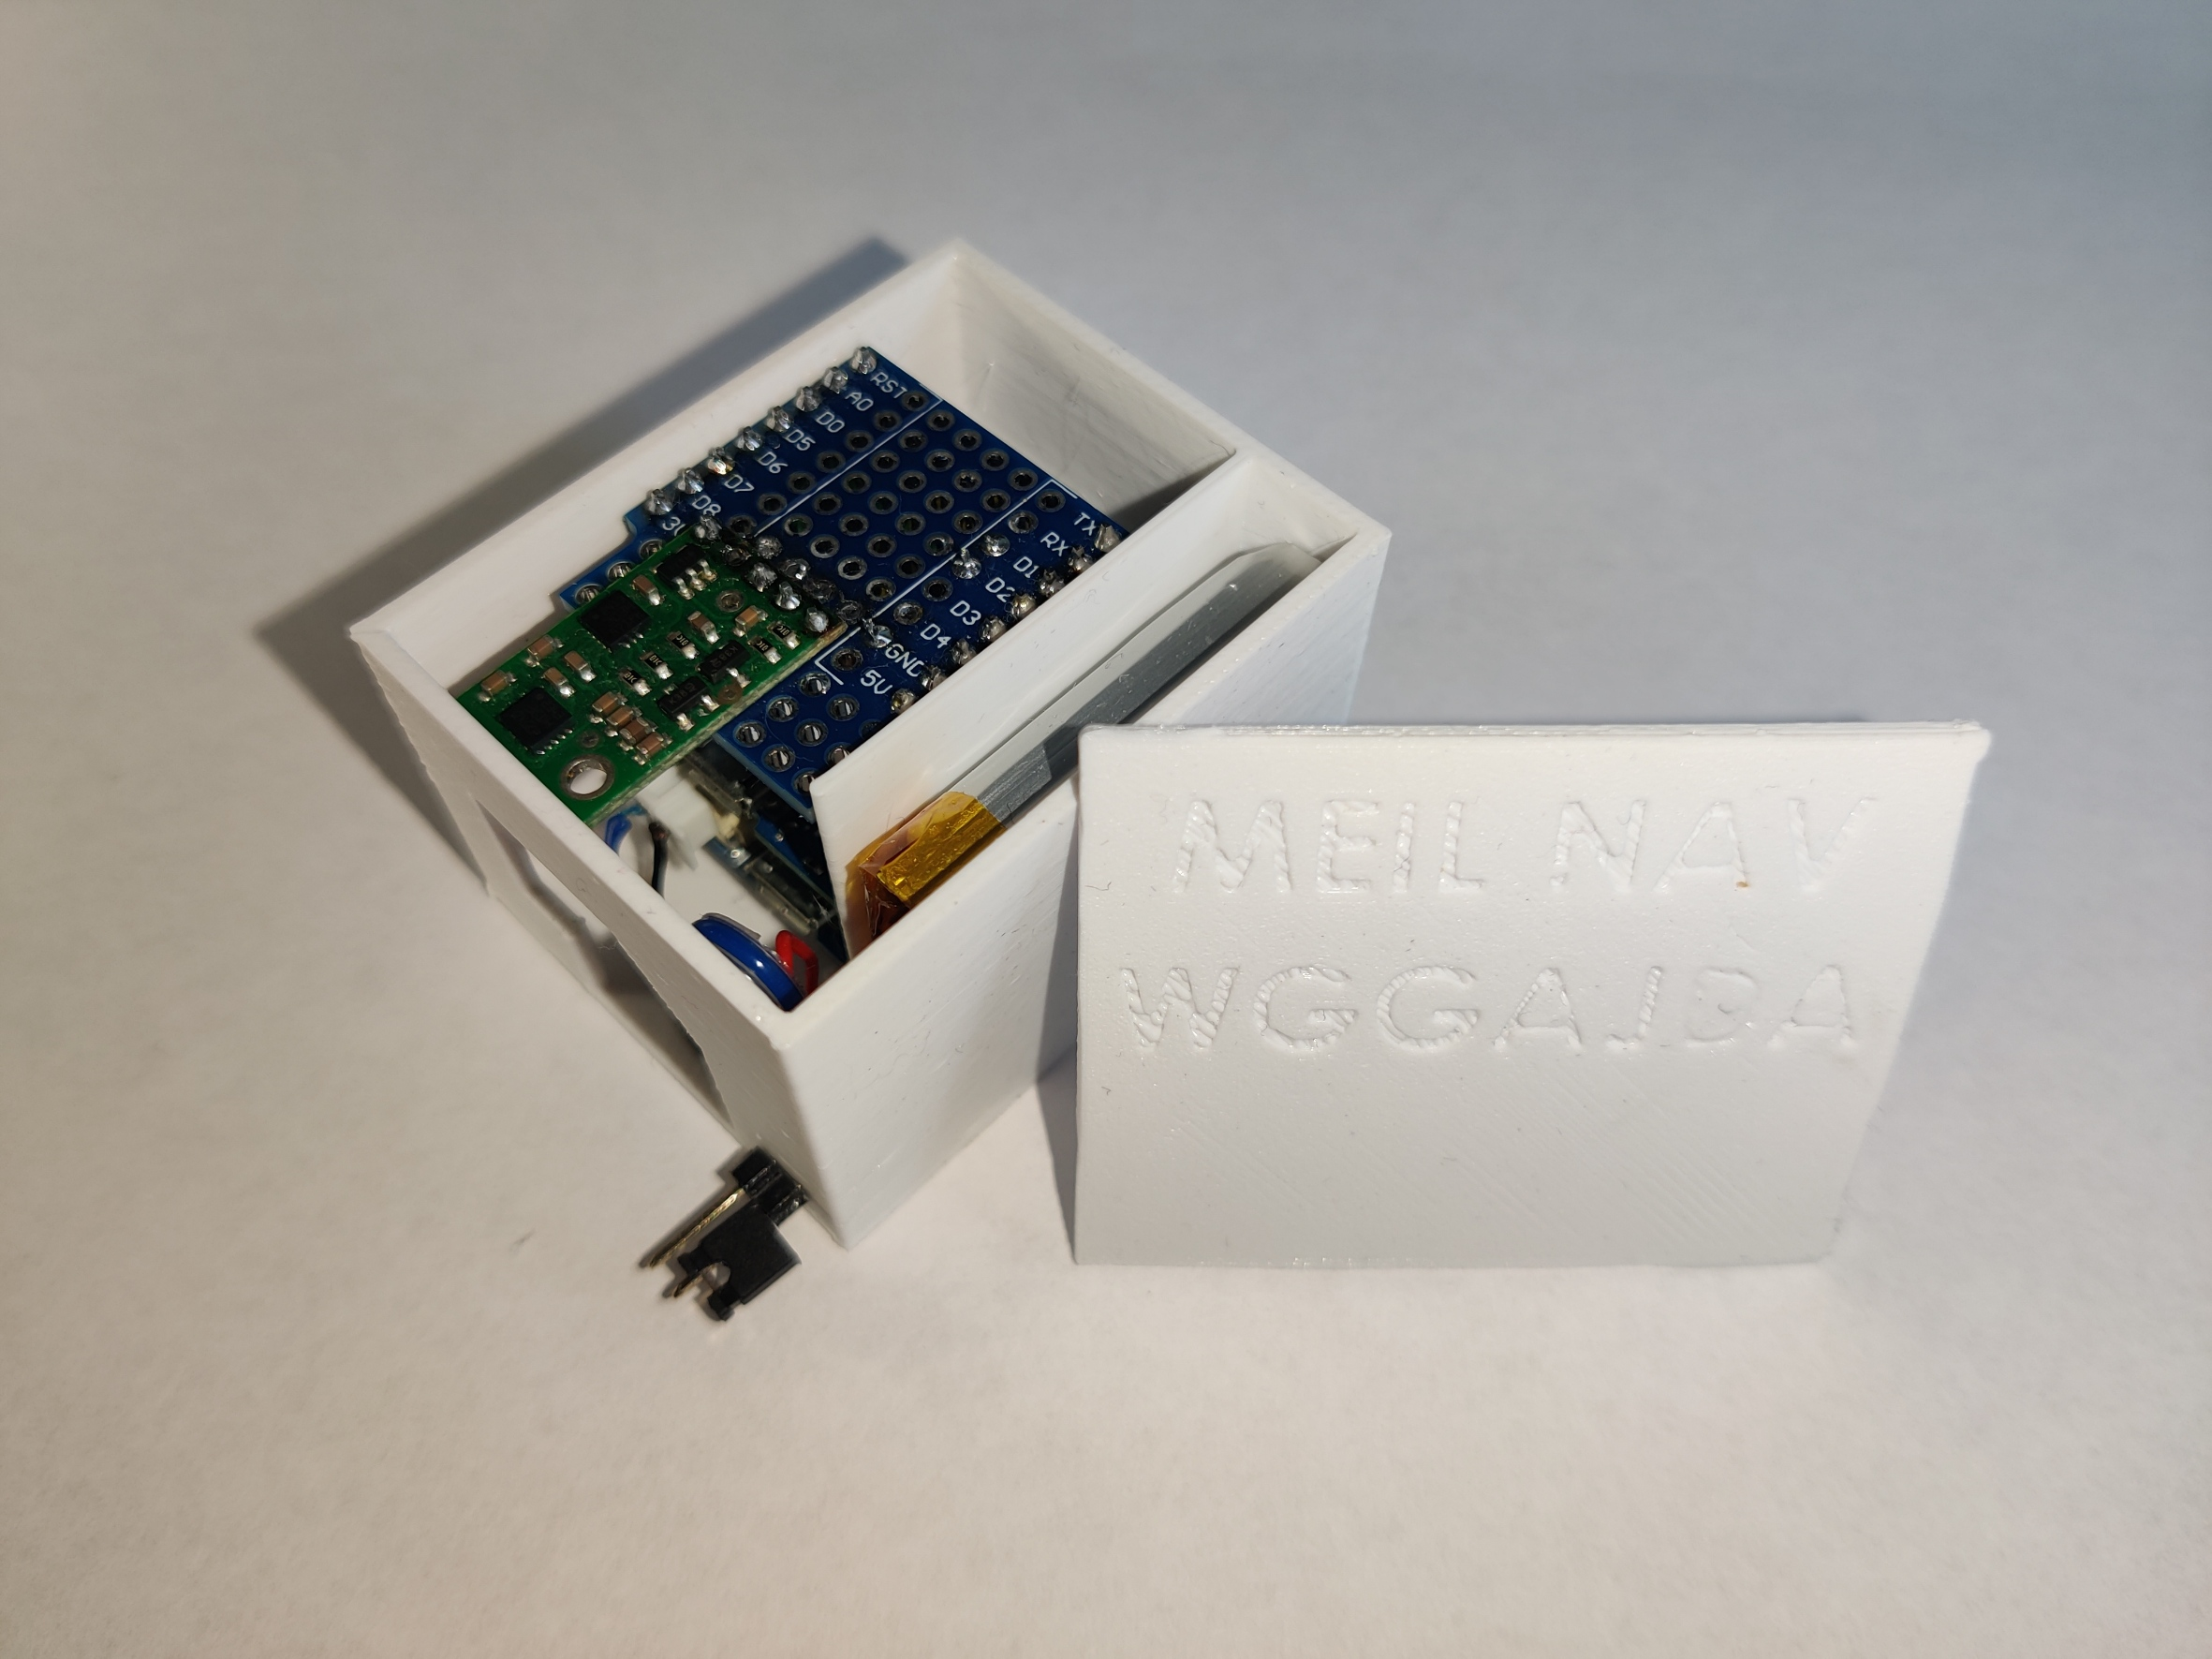
\includegraphics[width = 0.8\textwidth]{prototype.jpg}
	\end{center}
	\caption{Sensor node}
	\label{prototype}
\end{figure}

\renewcommand{\arraystretch}{1.2}
\begin{table}[!h]
	\centering
	\caption{Non-functional requirements -- FURPS}
	\label{furps}
	\begin{tabular}{|m{0.028\textwidth}|m{0.14\textwidth}|m{0.02\textwidth}|m{0.72\textwidth}|} 
		\hline
		\rowcolor{Gray}		\multicolumn{2}{|c|}{Requirement} & No. & Description \\
		\hline
		\centering \multirow{2.0}{*}{\rotatebox[origin=c]{90}{Usability}}
		&\multirow{1}{*}{Usability} 
		& 1 & The server runs natively on UNIX or in the Docker containter. The front-end application is multi-platform. \\
		\cline{2-4}
		& \multirow{1}{*}{Ergonomy} 
		& 2 & The user interface should be transparent and intuitive.  \\
		\cline{3-4}
		\hline
		\centering \multirow{2.0}{*}{\rotatebox[origin=c]{90}{Reliability}}
		& \multirow{1}{*}{Precision} 
		& 3 & The system should maximize estimation precision for collected readings. \\
		\cline{2-4}
		& \multirow{1}{*}{Verifiability} 
		& 4 & Estimation results should match predictions and be verifiable. \\
		\hline
		\centering \multirow{1}{*}{\rotatebox[origin=c]{90}{Perf.}}
		& \multirow{1}{*}{Performance} 
		& 5 & The system performance should scale relative to the number of sensors. \\
		\hline
		\centering \multirow{5.5}{*}{\rotatebox[origin=c]{90}{Supportability}}
		& \multirow{2}{*}{Maintenance} 
		& 6 & The system implementation should be transparent and easy to develop.  \\
		\cline{3-4}
		& & 7 & The system should be divided into modules that can be modified separately.\\
		\cline{2-4}
		& \multirow{1}{*}{Installability} 
		& 8 & The installation process should be easy. It is recommended for front-end software not to be installed. \\
		\cline{2-4}
		& \multirow{1}{*}{Configuration} 
		& 9 & Software should be magic-number-free, and all parameters should be configurable. \\
		\hline
	\end{tabular}
\end{table}

\section{Graphical user interface}

Figures \ref{gui1} - \ref{gui4} present graphical user interface of client module.

\begin{figure}[!h]
	\centering
	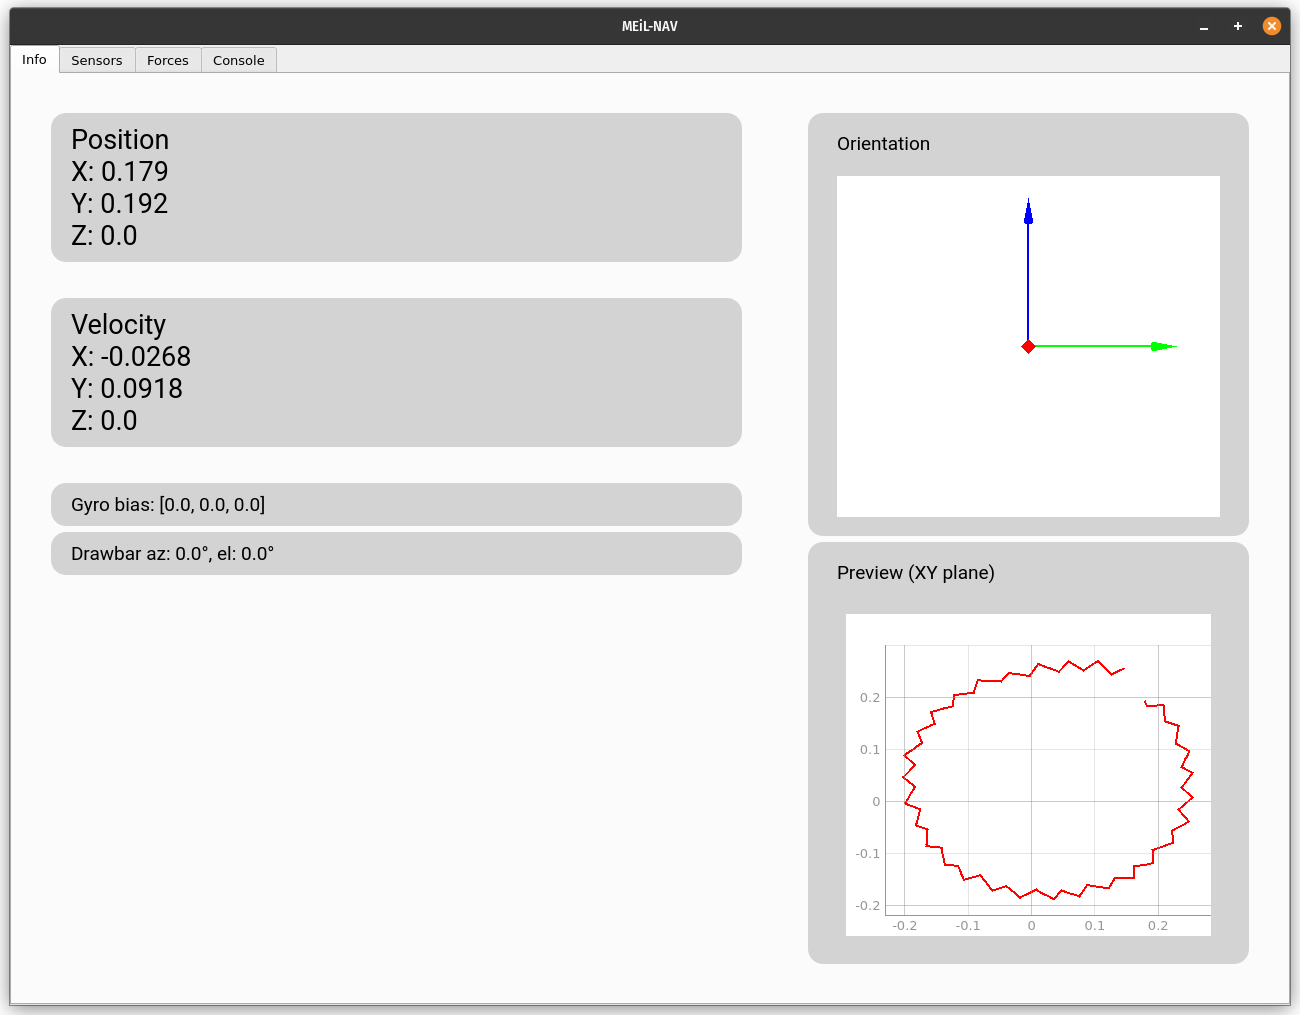
\includegraphics[width=0.8\textwidth]{gui_dashboard.png}
	\caption{GUI: the main dashboard}
	\label{gui1}
\end{figure}

\begin{figure}[!h]
	\centering
	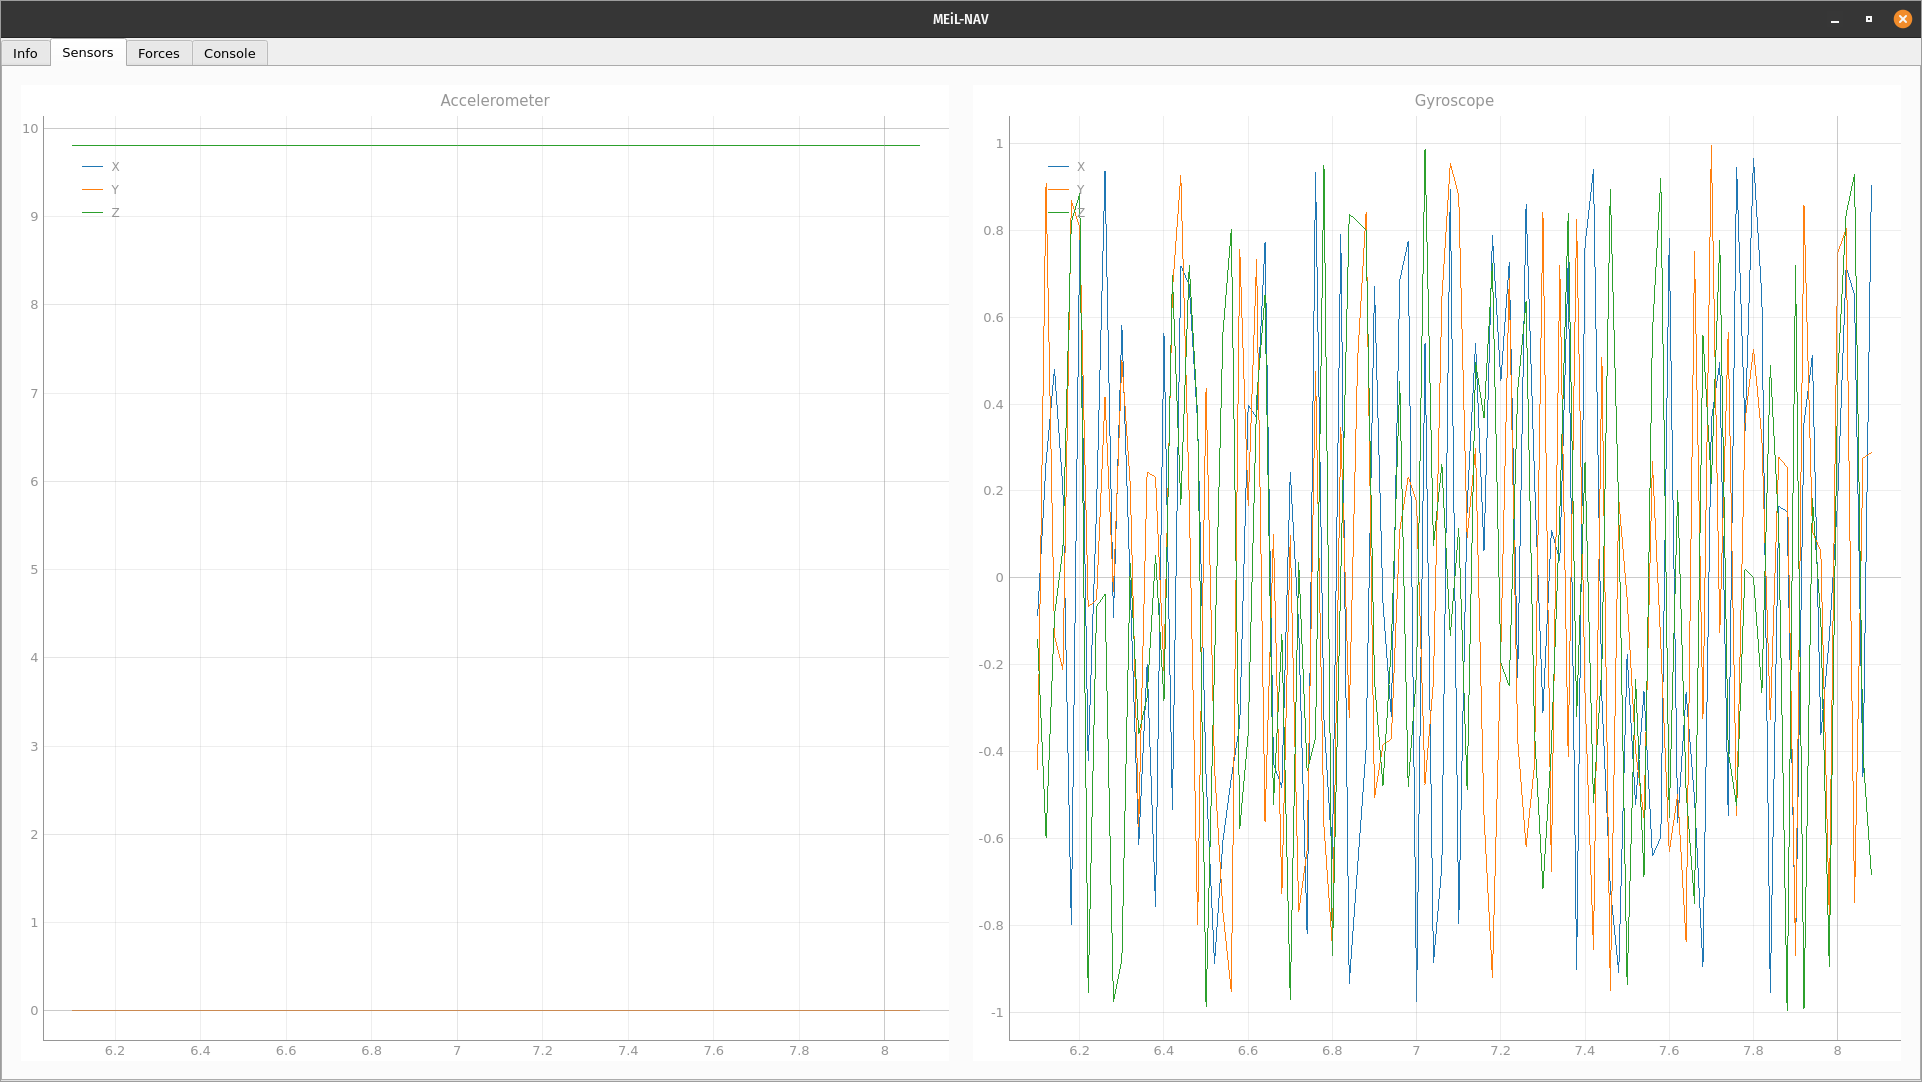
\includegraphics[width=0.8\textwidth]{gui_sensor.png}
	\caption{GUI: the sensor tab}
	\label{gui2}
\end{figure}

\begin{figure}[!h]
	\centering
	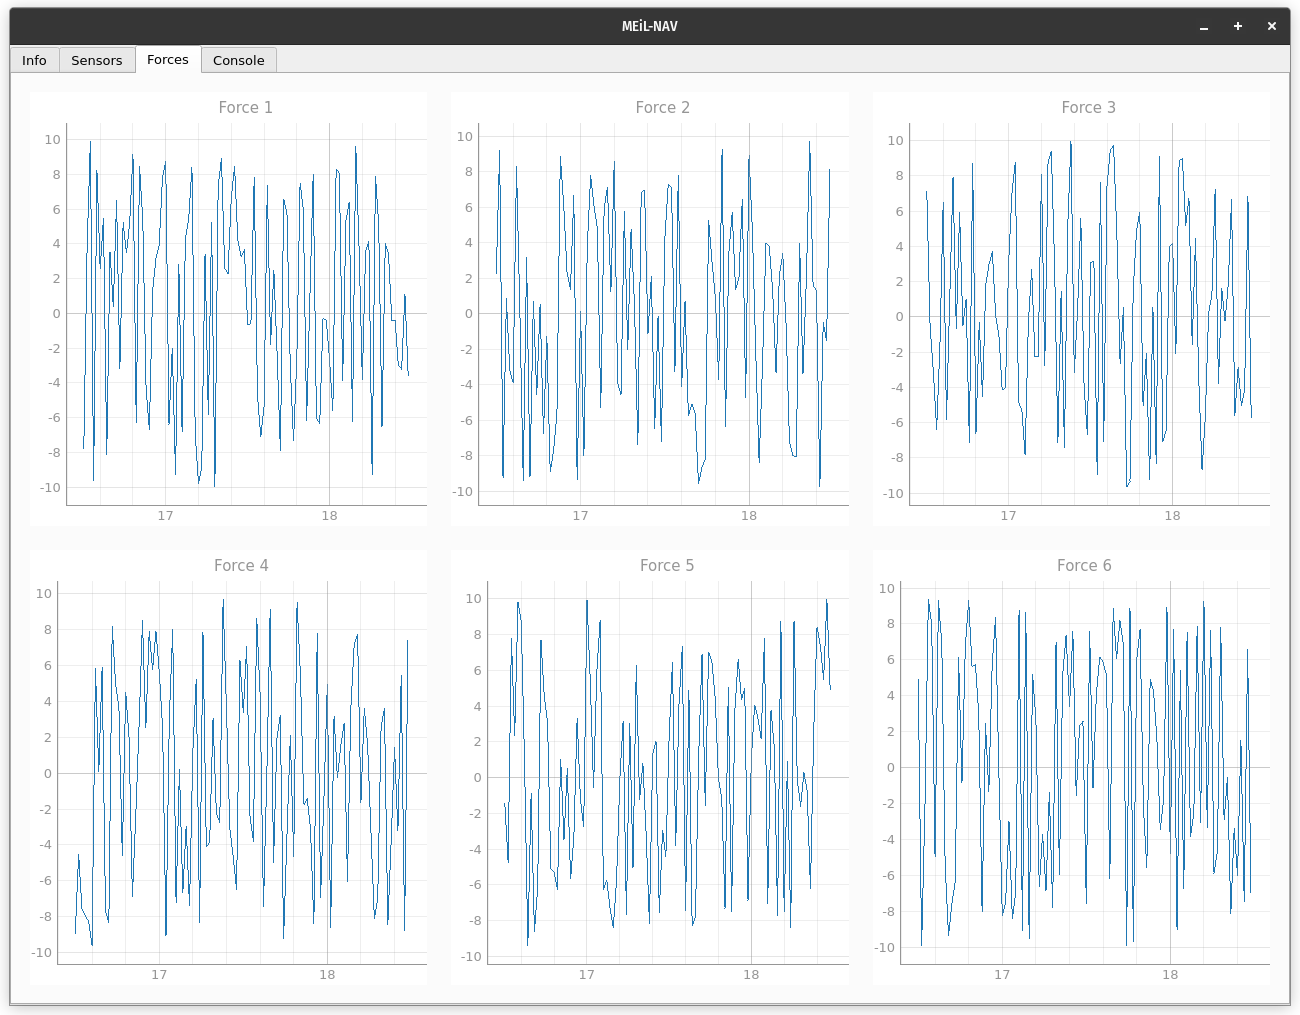
\includegraphics[width=0.85\textwidth]{gui_force.png}
	\caption{GUI: the force tab}
	\label{gui3}
\end{figure}

\begin{figure}[!h]
	\centering
	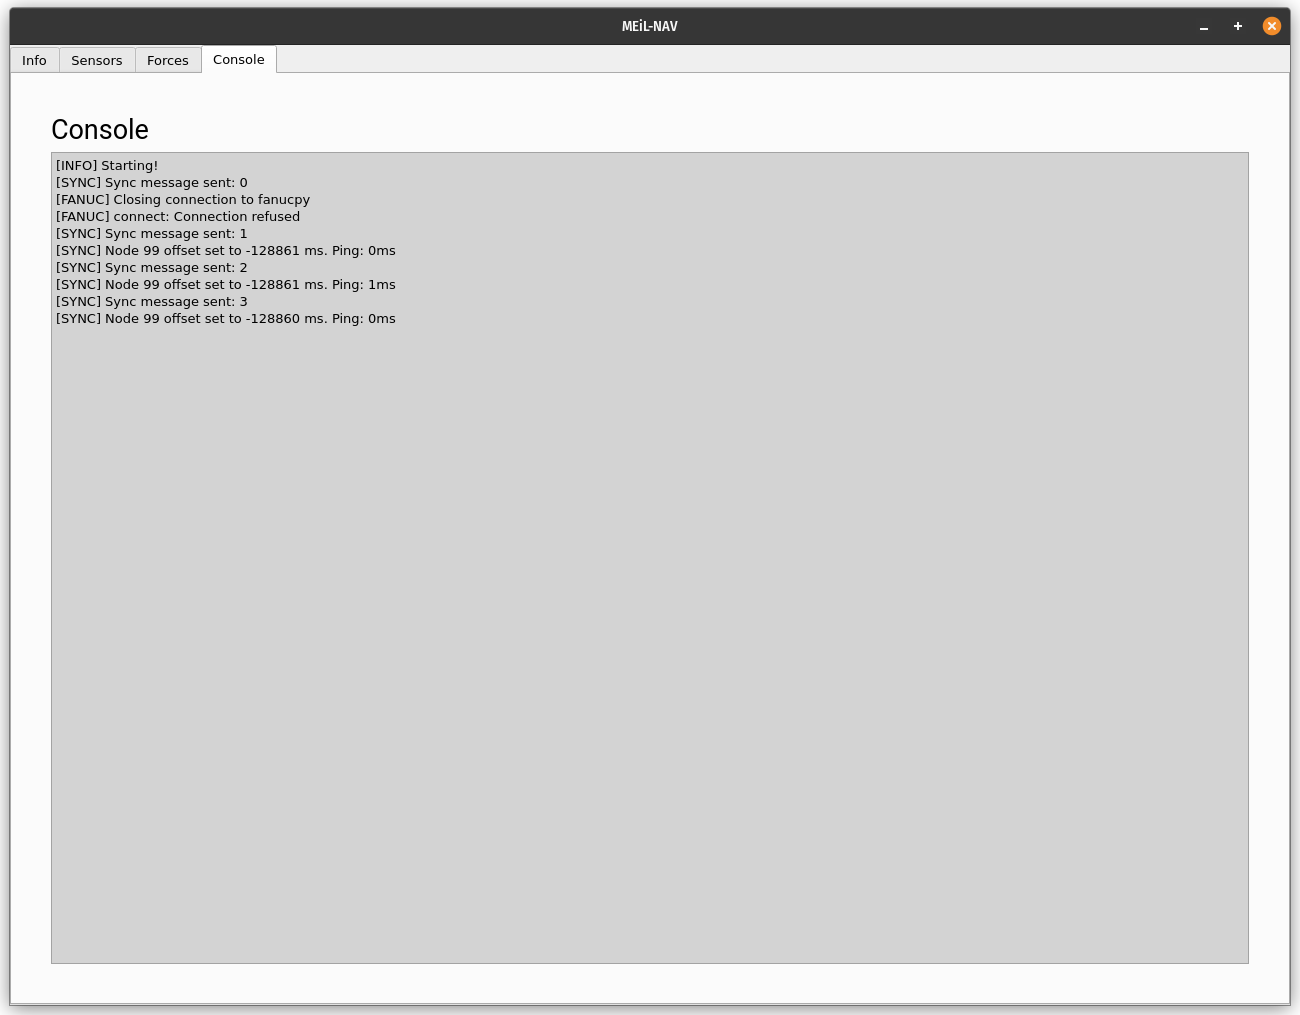
\includegraphics[width=0.85\textwidth]{gui_consol.png}
	\caption{GUI: the console tab}
	\label{gui4}
\end{figure}

\section{Plugins}

The developed software creates an advanced multitask system. During its preparation there was a lot of attention paid to make software flexible and easily updated. This allows you to enrich the system with features needed for specific applications. Those addons, that are not strictly connected with system's main task are called plugin.\\

An example of plugin, that was added to system is force logger. The main task of this plugin is collecting data from tension transducer connected via MODBUS TCP. For this purpose force logger utilizes already implemented timestamp system and save logs in project's specific format. Stored data are also synchronized with other estimations.

\section{Tuning}

Tuning is a process of selecting the set of parameters that provides the best results in terms of the chosen criterion. For the system being developed, the greatest number of unknowns are the parameters of sensor filtration and fusion. Based on similar projects and applications, the initial value of parameters can be selected, but tuning is an unmissable step on the way to precise estimation.\\

In measurement systems, the final result is affected by almost every element of the system: sensor errors, installation errors, delays, and more. Due to that, there is no universal method of tuning. The process largely depends on the operator's experience and ability to recognize system responses. Nevertheless, it is prolific to plan experiments that highlight certain regions of interest and, as a result, lead to shorter tuning times.\\

The project took care to include all the parameters in a configuration file that is freely editable. Parameters were divided into categories, and a few of them can be modified on-line, when the system runs. The source code is devoid of modifiable numerical constants (so-called \textit{magic numbers}). Additionally, the configuration file contains software variables that define network topology, addressing and other parameters that are configured during deployment.

